\subsection{A/D-Wandlerchip ADC0804} % (fold)
\label{sub:A/D-Wandlerchip_ADC0804}
\begin{frame}
    \frametitle{A/D Wandlerchip}
    \framesubtitle{}
    \begin{figure}[H]
    \begin{center}
            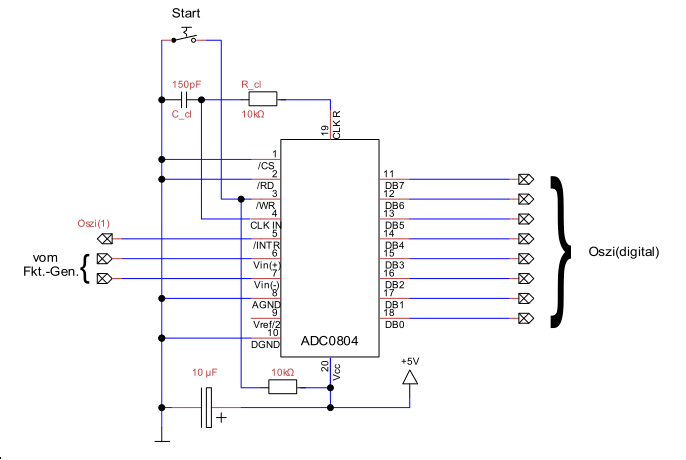
\includegraphics[scale=0.4]{./img/schaltung/ADWandler_0.png}
    \end{center}
    \end{figure}
\end{frame}

\begin{frame}
    \frametitle{Theorie}
    \framesubtitle{}
    \begin{block}{Theoretischer Wert}
        \begin{itemize}
            \item Aufteilung der Spannung $V_{cc}$ in 255 Teile
        \end{itemize}
            \begin{gather*}
                U_{out} = \frac{n}{255} \cdot V_{cc} \\
                n = \left\lfloor \frac{U_{out}}{V_{cc}} \cdot 255 \right\rfloor
            \end{gather*}
    \end{block}
\end{frame}

\begin{frame}
    \frametitle{Messwerte}
    \framesubtitle{}
            \begin{figure}[H]
            \begin{center}
                    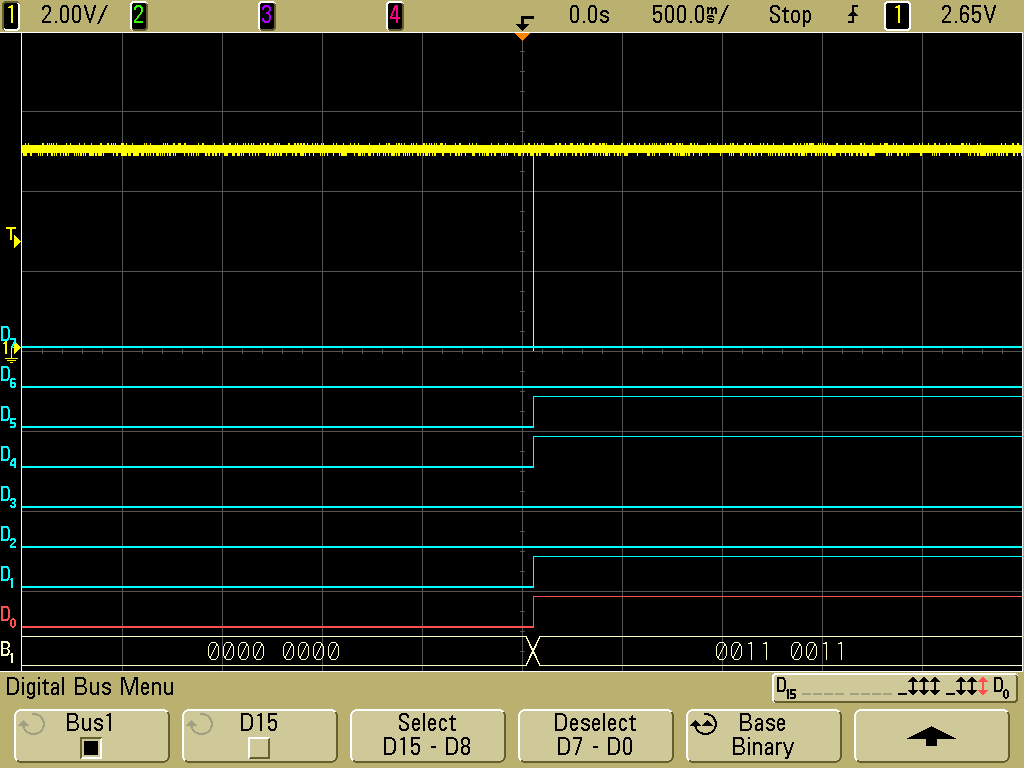
\includegraphics[scale=0.2]{./img/oszi/scope_10.png}
            \end{center}
            \end{figure}
            \begin{center}
            \boxed{
                \begin{tabular}{c|c|c|c}
                    $U$ & Bin & Dez & Theorie\\
                    \hline
                    $1V$ & $00110011$ & $51$ & $51$
                \end{tabular}
                }
            \end{center}
\end{frame}


\begin{frame}
    \frametitle{Messwerte}
    \framesubtitle{}
            \begin{figure}[H]
            \begin{center}
                    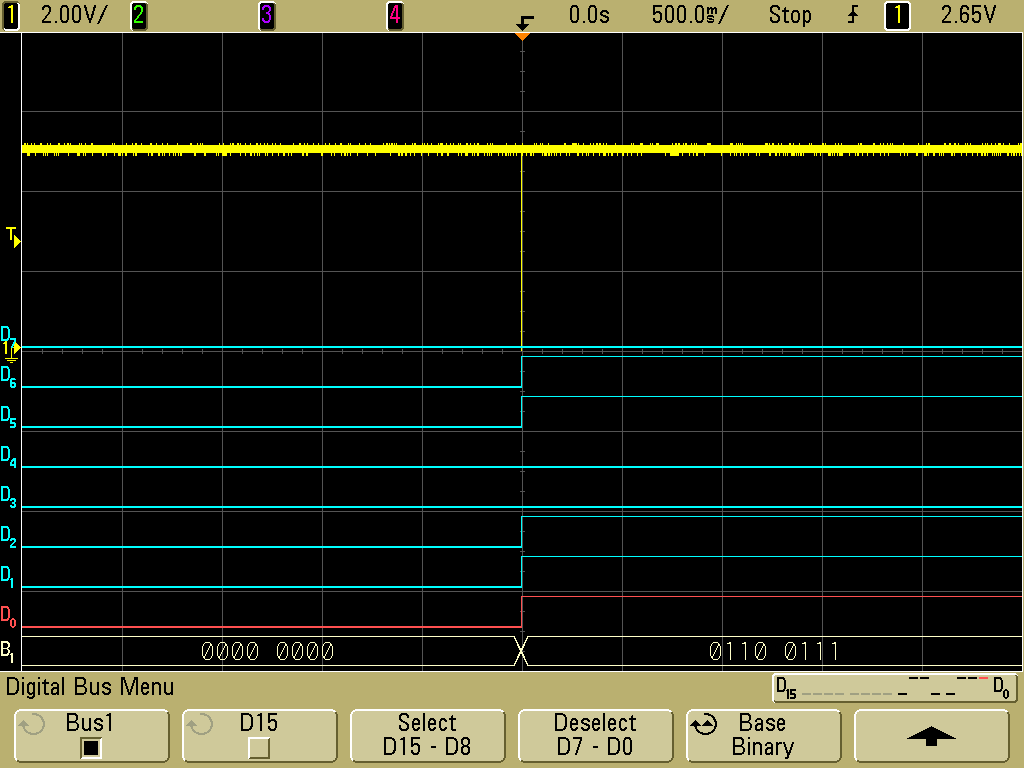
\includegraphics[scale=0.2]{./img/oszi/scope_9.png}
            \end{center}
            \end{figure}
            \begin{center}
            \boxed{
                \begin{tabular}{c|c|c|c}
                $U$ & Binl & Dez & Theorie\\
                \hline
                $1V$ & $00110011$ & $51$ & $51$ \\
                $2V$ & $01100111$ & $103$ & $102$ 
                \end{tabular}
                }
            \end{center}
\end{frame}

\begin{frame}
    \frametitle{Messwerte}
    \framesubtitle{}
            \begin{figure}[H]
            \begin{center}
                    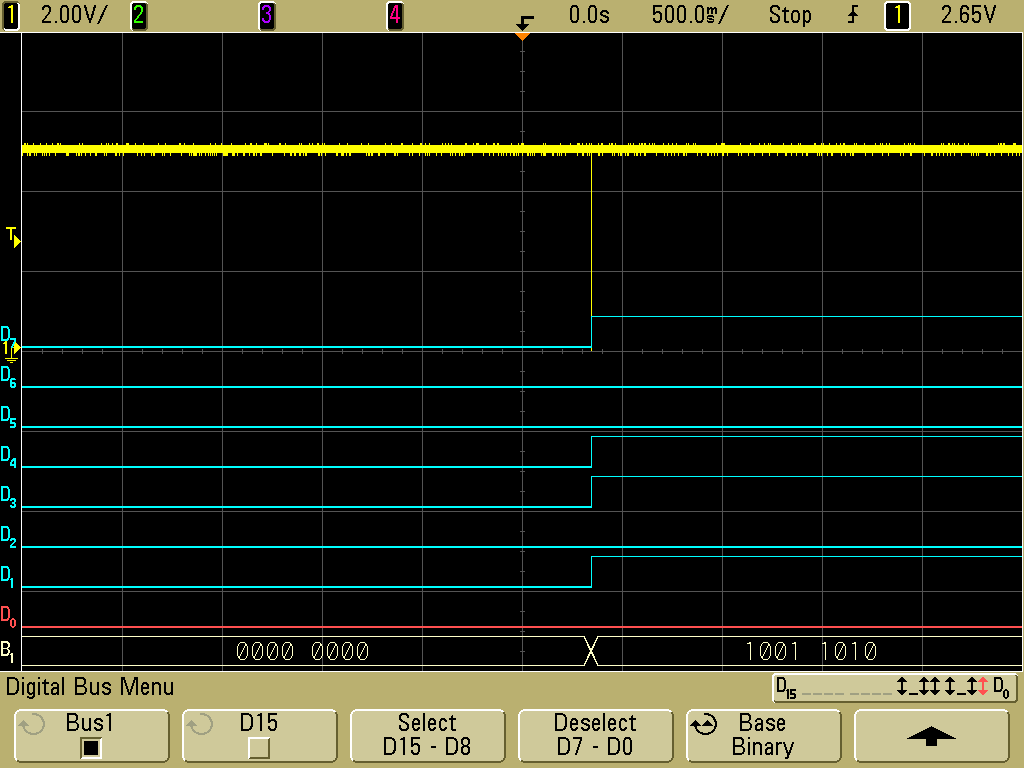
\includegraphics[scale=0.18]{./img/oszi/scope_11.png}
            \end{center}
            \end{figure}
            \begin{center}
            \boxed{
                \begin{tabular}{c|c|c|c}
                $U$ & Bin & Dez & Theorie\\
                \hline
                $1V$ & $00110011$ & $51$ &$51$\\
                $2V$ & $01100111$ & $103$&$102$ \\
                $3V$ & $10011010$ & $154$&$153$ 
                \end{tabular}
                }
            \end{center}
\end{frame}

\begin{frame}
    \frametitle{Umbau}
    \framesubtitle{}
    \begin{columns}[c]
        \column{0.4\textwidth}
            \begin{block}{}
                \begin{itemize}
                    \item Widerstand zwischen $20$ und $3$ wird zwischen $3$ und $5$
                    eingebaut
                    \item sobal INTR Spannung ausgibt wird der Wandlungsprozess
                    durch WR neu gestartet
                    \item geeignet für Wechselspannung
                \end{itemize}
            \end{block}
        \column{0.6\textwidth}
            \begin{figure}[H]
            \begin{center}
                    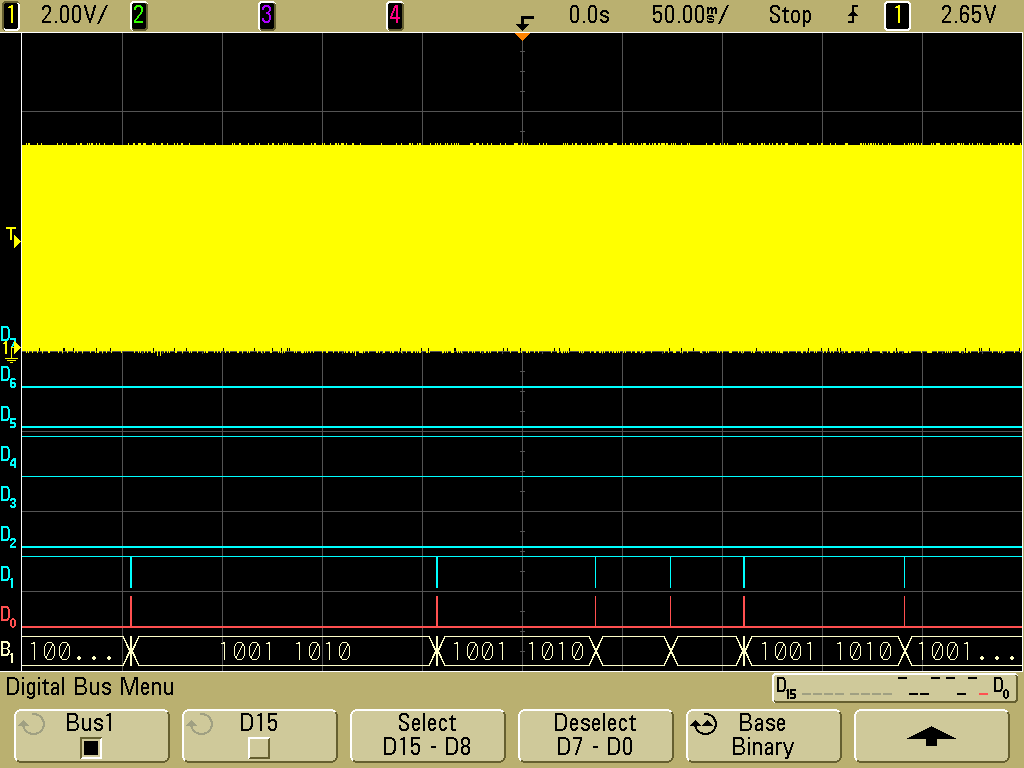
\includegraphics[scale=0.12]{./img/oszi/scope_12.png}
            \end{center}
            \end{figure}
            \begin{figure}[H]
            \begin{center}
                    %\includegraphics[scale=0.1]{./img/schaltung/ADC_0.png}
            \end{center}
            \end{figure}
    \end{columns}
\end{frame}
\begin{frame}
    \frametitle{Sinusfunktion}
    \framesubtitle{100Hz}
     \begin{figure}[H]
     \begin{center}
             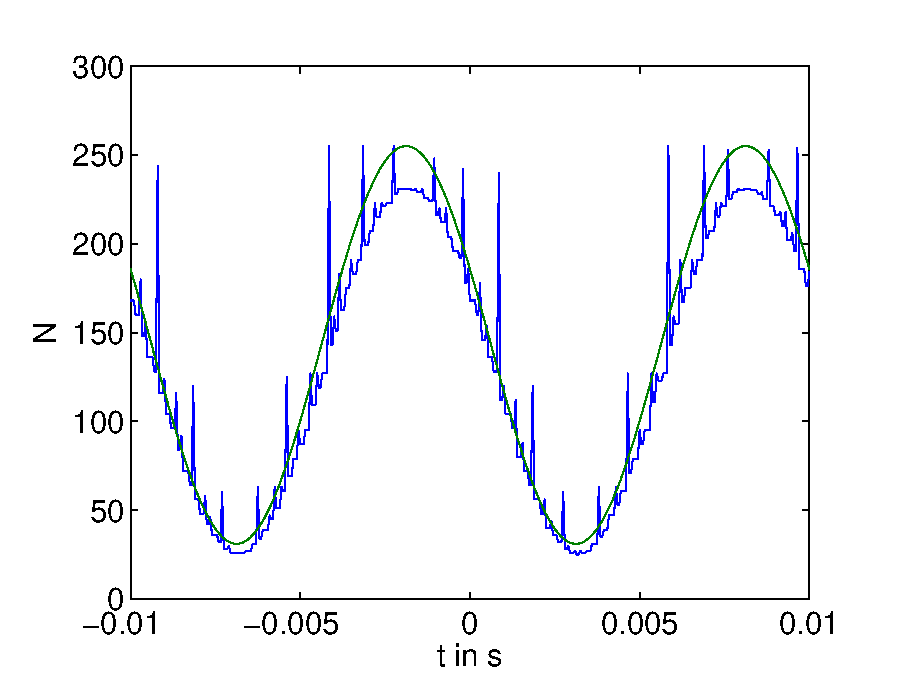
\includegraphics[scale=0.5]{./img/graph/Aufgabe3_100hz_N.eps}
     \end{center}
     \end{figure}
\end{frame}
\begin{frame}
    \frametitle{Sinusfunktion}
    \framesubtitle{1kHz}
     \begin{figure}[H]
     \begin{center}
             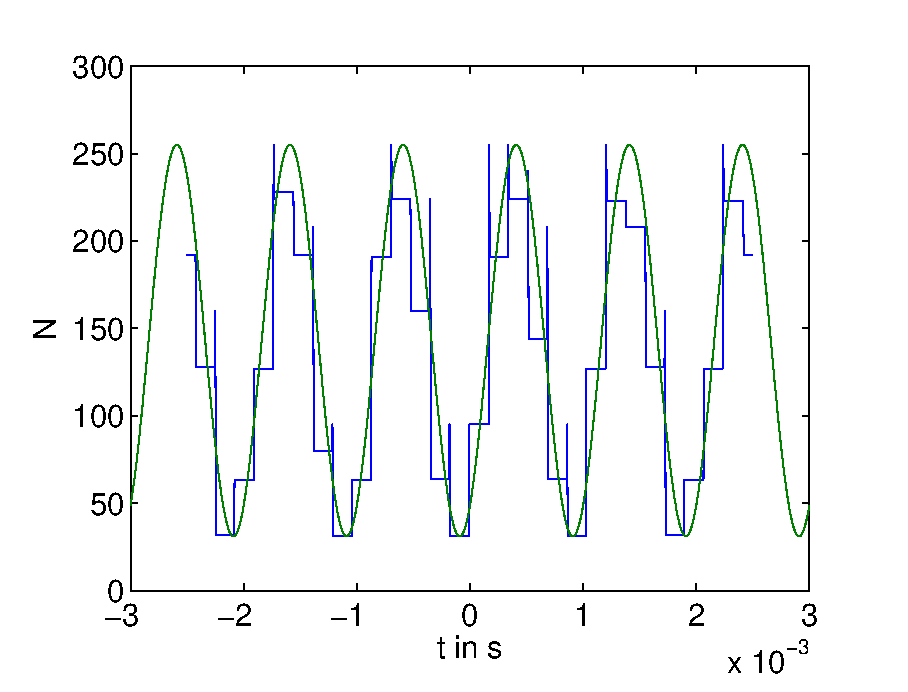
\includegraphics[scale=0.5]{./img/graph/Aufgabe3_1khz_N.eps}
     \end{center}
     \end{figure}
\end{frame}
\begin{frame}
    \frametitle{Sinusfunktion}
    \framesubtitle{4khz}
     \begin{figure}[H]
     \begin{center}
             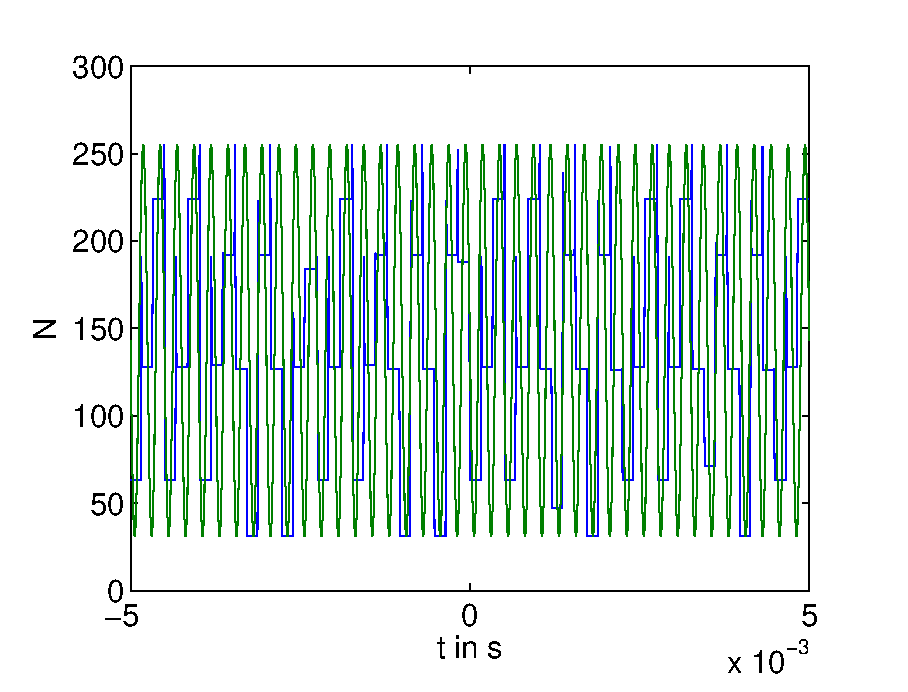
\includegraphics[scale=0.5]{./img/graph/Aufgabe3_4khz_N.eps}
     \end{center}
     \end{figure}
\end{frame}
\begin{frame}
    \frametitle{Sinusfunktion}
    \framesubtitle{10kHz}
     \begin{figure}[H]
     \begin{center}
             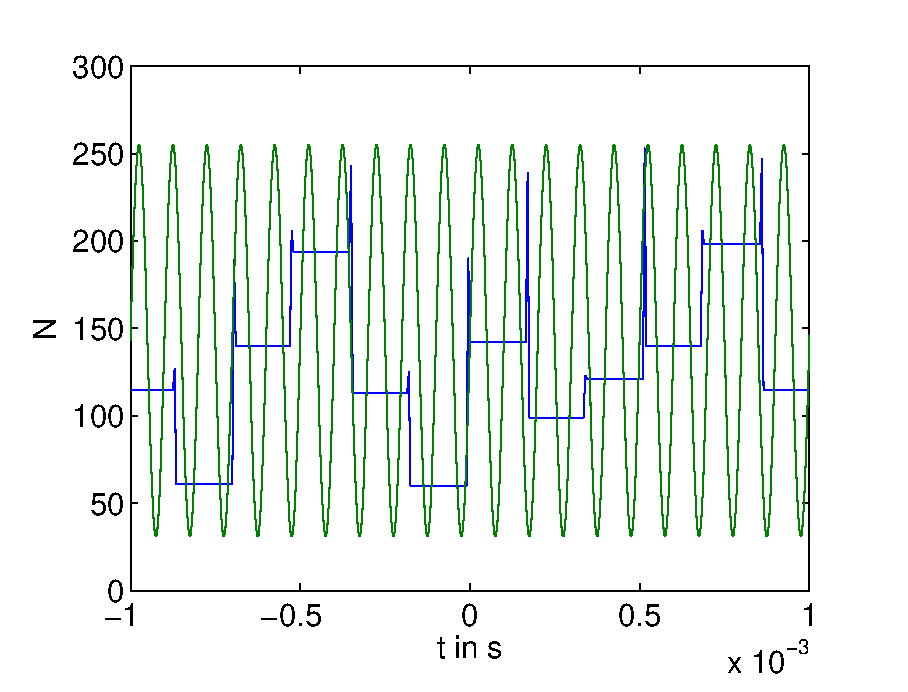
\includegraphics[scale=0.5]{./img/graph/Aufgabe3_10khz_N.eps}
     \end{center}
     \end{figure}
\end{frame}
\begin{frame}
    \frametitle{Ergebnis}
    \framesubtitle{}
    \begin{columns}[c]
        \column{0.5\textwidth}
             \begin{figure}[H]
             \begin{center}
                     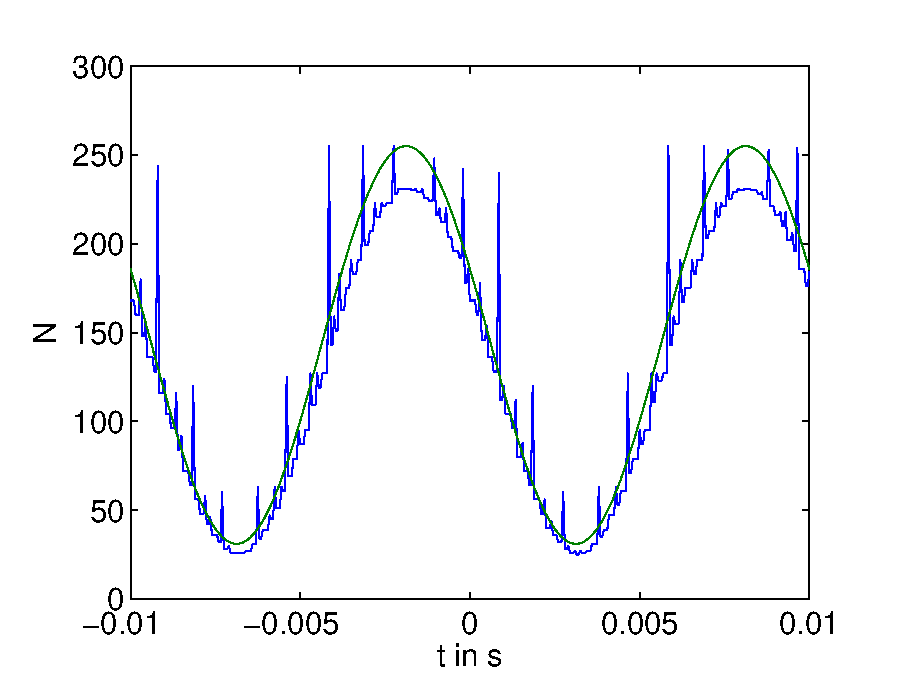
\includegraphics[scale=0.3]{./img/graph/Aufgabe3_100hz_N.eps}
             \end{center}
             \caption{100Hz}
             \end{figure}
        \column{0.5\textwidth}
             \begin{figure}[H]
             \begin{center}
                     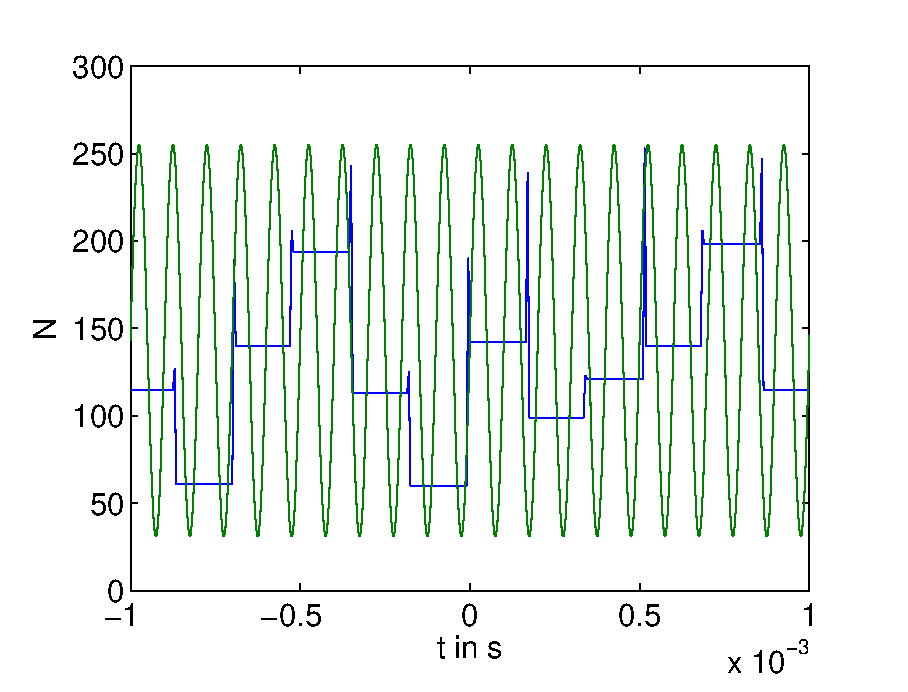
\includegraphics[scale=0.3]{./img/graph/Aufgabe3_10khz_N.eps}
             \end{center}
             \caption{10kHz}
             \end{figure}
    \end{columns}
     \begin{block}{}
         \begin{itemize}
             \item Je höher die Referenzfrequenz, desto Ungenauer wird die
             Wandlung
             \item Kurve kann nicht mehr ausreichend abgetastet werden
         \end{itemize}
     \end{block}
\end{frame}
\begin{frame}
    \frametitle{Wandlungsrate}
    \framesubtitle{}
    \begin{columns}[c]
        \column{0.5\textwidth}
            \begin{block}{Wandlungsrate}
                \begin{itemize}
                    \item Aus Messung:  
                    \begin{equation*}
                        f_s = 5.7kHz
                    \end{equation*}
                \end{itemize}
            \end{block}
        \column{0.5\textwidth}
            \begin{figure}[H]
            \begin{center}
                    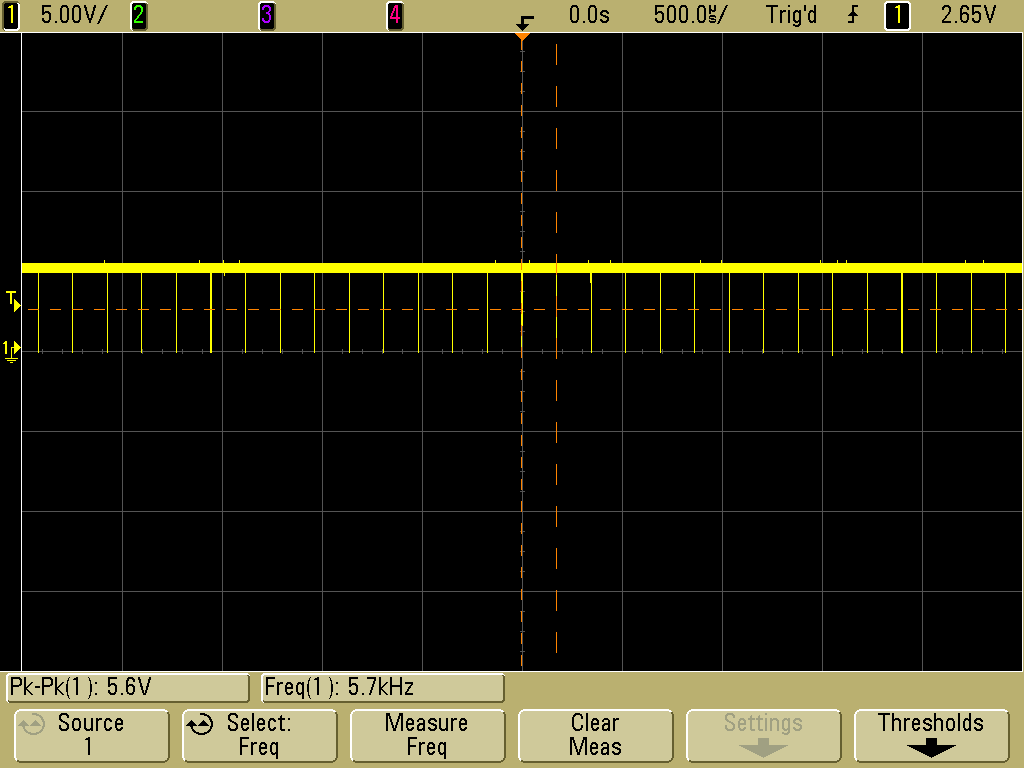
\includegraphics[scale=0.15]{./img/oszi/scope_13.png}
            \end{center}
            \end{figure}
    \end{columns}
\end{frame}
\begin{frame}
    \frametitle{Störung}
    \framesubtitle{}
    \begin{columns}[c]
        \column{0.4\textwidth}
            \begin{block}{}
                \begin{equation*}
                    f_s = \frac{1}{1.1 \cdot R \cdot C}
                \end{equation*}
            \begin{itemize}
                \item Körperkontakt verringert Kapazität $\rightarrow$
                Vergrößerung der Abtastrate
            \end{itemize}
            \end{block}
        \column{0.6\textwidth}
        \begin{figure}[H]
        \begin{center}
                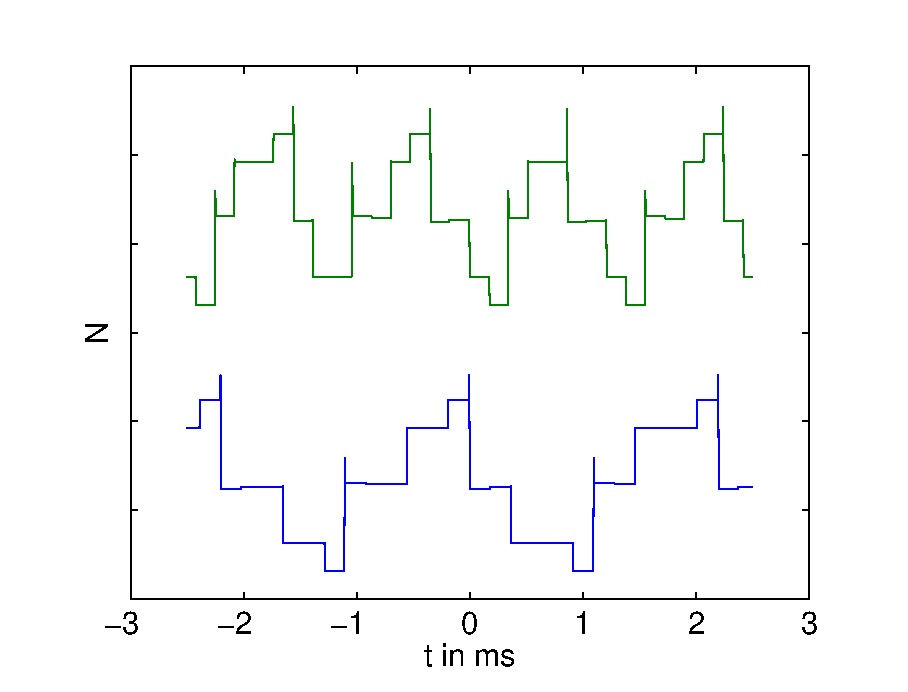
\includegraphics[scale=0.4]{./img/graph/Aufgabe3_Druck_N.eps}
        \end{center}
        \end{figure}
    \end{columns}
    
\end{frame}
